Legacy outlines enter the system through a normalization step that converts several human-friendly forms into the same canonical work representation. The goal is not merely to parse text, but to preserve authorial intent while making the structure machine-readable, comparable, and ready for downstream coordination. In practice, the importer accepts legacy YAML, markdown headers, numbered outlines, and even raw prose notes, then rewrites them into the work-oriented YAML used by the rest of the repository.

The normalization process begins by identifying the source shape. A legacy YAML file may already contain nested nodes, titles, and summaries, but its field names, nesting conventions, or metadata layout may differ from the current schema. Markdown sources usually encode structure implicitly through heading levels, list indentation, and emphasis. Numbered outlines often express hierarchy through numbering patterns such as 1, 1.1, and 1.1.1. Raw text may contain only paragraphs or loosely separated notes, requiring the importer to infer section boundaries from formatting cues and surrounding context. Each of these inputs is treated as a different surface form of the same underlying authorial plan.

Normalization then maps the imported material into canonical work YAML. At the top level, the importer establishes the work root and ensures that the document has the fields expected by the rest of the system: title, summary, intent, metadata, and a recursive structure of chapters, sections, and subsections. Imported headings become structural nodes with stable identifiers and explicit numbers. Free-form notes are attached as summaries or content files where appropriate, rather than left as ambiguous inline text. When the source already contains a usable hierarchy, the importer preserves that hierarchy while regularizing names, numbering, and field placement so that later agents can reason over it consistently.

A key part of the process is structural normalization. Markdown heading depth is translated into the book's recursive outline tree, with heading levels converted into chapter, section, or subsection nodes as needed. Numbered outlines are similarly converted by reading the numbering as a hierarchy signal rather than as presentation text. If the source uses mixed conventions, the importer resolves them into a single tree and records the result in a form that can be traversed uniformly. This makes it possible for later stages to compare sibling sections, detect missing dependencies, and generate section payloads without special-case parsing for each source format.

The importer also normalizes content boundaries. Some legacy sources place prose directly under headings, while others mix outline text with draft paragraphs or editorial notes. The canonical form separates structure from payload: the outline describes what exists, and the section content file or section body carries the prose that belongs to that node. This separation is important because the system treats the outline as durable project state, while section payloads are generated or revised independently. By moving imported text into the appropriate structural slot, the importer prevents accidental duplication and makes later revisions easier to target.

When the source is underspecified, normalization favors conservative preservation over invention. Raw text that cannot be confidently split into multiple sections should remain grouped rather than being over-partitioned. Ambiguous labels should be retained in a way that allows human review. The importer should not fabricate missing claims, dependencies, or metadata; instead, it should produce the most faithful canonical representation possible and leave unresolved gaps visible for later editorial work. In this sense, normalization is a migration step, not a creative rewrite.

The output of import is therefore a canonical work YAML file that can serve as the system's shared source of truth. Once normalized, the outline can be consumed by section agents, gardener checks, reference workflows, and build tooling without needing to know whether the project began as a legacy YAML tree, a markdown document, a numbered outline, or a block of raw notes. The importer turns heterogeneous author input into a stable project object, and that stability is what allows the rest of the machine to coordinate around a single representation.

In the repository's workflow, this section sits between conversational intake and repository layout. Conversational intake captures intent from the author; outline import converts preexisting material into the same canonical shape; repository layout then determines where the resulting work object, section payloads, logs, and artifacts live. Together, these steps define the path from informal source material to a structured book project that the rest of the Codynamic Book Machine can maintain.

\begin{figure}[htbp]
\centering
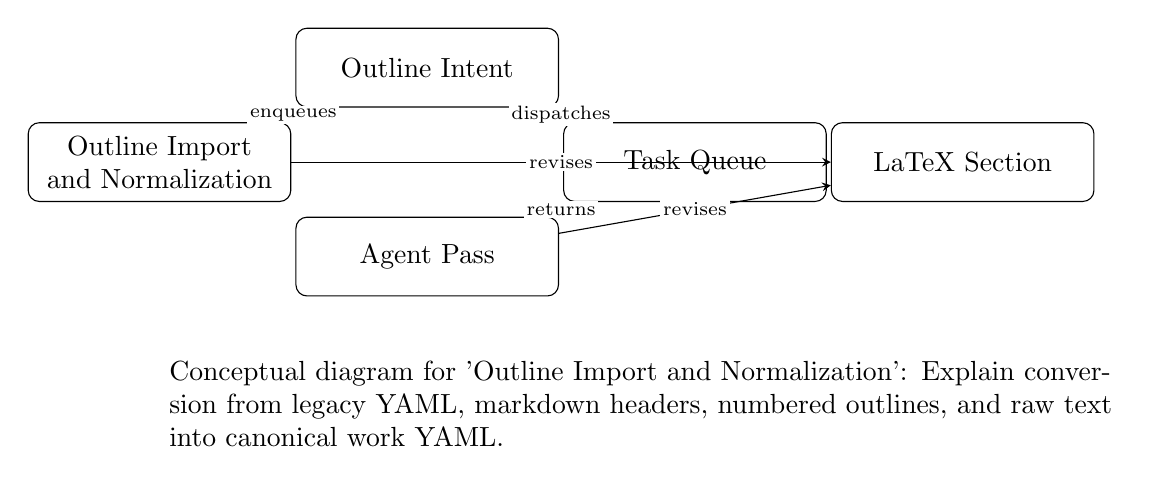
\begin{tikzpicture}[>=stealth, node distance=2.2cm,
  concept/.style={draw, rounded corners, align=center, text width=3.1cm, minimum height=1cm},
  relation/.style={font=\scriptsize, fill=white, inner sep=1pt}]
\node[concept] (n1) at (0,0) {Outline Import and Normalization};
\node[concept] (n2) at (3.4,1.2) {Outline Intent};
\node[concept] (n3) at (6.8,0) {Task Queue};
\node[concept] (n4) at (3.4,-1.2) {Agent Pass};
\node[concept] (n5) at (10.2,0) {LaTeX Section};
\draw[->] (n1) -- node[relation] {enqueues} (n2);
\draw[->] (n2) -- node[relation] {dispatches} (n3);
\draw[->] (n3) -- node[relation] {returns} (n4);
\draw[->] (n4) -- node[relation] {revises} (n5);
\draw[->] (n1) -- node[relation] {revises} (n5);
\node[align=left, text width=12cm, anchor=north west] at (0,-2.4) {Conceptual diagram for 'Outline Import and Normalization': Explain conversion from legacy YAML, markdown headers, numbered outlines, and raw text into canonical work YAML.};
\end{tikzpicture}

\caption{Conceptual diagram for ``Outline Import and Normalization'': Explain conversion from legacy YAML, markdown headers, numbered outlines, and raw text into canonical work YAML.}
\end{figure}
